\documentclass{report}
\usepackage{blindtext}
\usepackage[utf8]{inputenc}
\usepackage{algorithm}
\usepackage[noend]{algpseudocode}
\usepackage{titlesec}
\usepackage{mathtools}
\usepackage{tikz} %% Package for drawing finite state machines in LaTEX
\usetikzlibrary{automata, positioning,arrows}
\newcommand{\me}[1]{
\begin{math}
#1
\end{math}
}
\title{Home Work 3}
\author{Francisco J. Díaz Riollano \\ Student ID: 802-15-2172 }


\begin{document}

\maketitle
 %%%%%%%%%%%%%%%%%%% First Question%%%%%%%%%%%%%%%%%%%%%%%
\paragraph{\Large{Question 1\\ \\}}


\begin{algorithm}
  \begin{algorithmic}[1]
    \Procedure{NAIVE}{\textit{On input} S[1,..m]}
      \State $n\gets |T|$
      \State $m\gets |S|$
      \For{s=0 \textbf{to} n-m}
      \If{P[1,..m] = T[s+1...s+m]}
      	\State \textbf{print}\textit{(``pattern found")}
      \EndIf
      \EndFor     
    \EndProcedure
  \end{algorithmic}
\end{algorithm}


The string matching problem is defined as: "Given a text \me{T=T_1 ... T_n} which is stored as array \me{T= T[1,...,n]} , and a pattern \me{P = P_1 ... P_m = P[1...m]} with \me{m<n}, where both are strings over the same alphabet \me{\Sigma;}decide whether S is a substring of T.

Algorithm 1 is the so-called naive-pattern finding algorithm. Use Algorithm 1 to construct a Finite State. Automata(deterministic or non-deterministic) for solving the matching problem. 
\\

Let M \me{=(Q,\Sigma,\delta,q_0,F)} be 5-tuple NFSA where: \newline
Q is a finite set of states \newline
\me{\Sigma} is a finite set if input symbols \newline
\me{\delta} is a state transition function from \me{Q \times \Sigma \rightarrow Q} \newline
\me{q_0 \in Q} is the initial state \newline
\me{F \subseteq Q} Q is the set of final states \newline
Let \me{\Sigma=\{s_1,s_2,...,s_{|A|}\}} for the alphabet of the input string and the text. \newline
\\
\\
High Level Description of the automata: \\
M =: ``On input S[1,...,m]" \\
1) Read the input strings S. \\
2) The automata checks if the string that is being read matches.
3) Otherwise it loops to the state of the closest seen pattern \\
4) If there is no previous seen pattern it loops to the start state\\
5) If the string read matches the $P_jth$ pattern then continue to the $P_{j+1}th$ pattern state.\\
6) If all the pattern states have been visited, then this implies that a pattern has been found thus the machine ``accepts".\\

An simple example:
Let  M be a machine such that it describes the pattern \me{P = ``021"}.\newline
 \me{\Sigma =\{0,1,2\}, Q =\{q_0,q_1,q_2\}}. For the given pattern the Automata look as such.
\\ \\ \\
% %%%%%%%%%%%%%%%%Automata Describing the algorithm %%%%%%%%%%%%%%
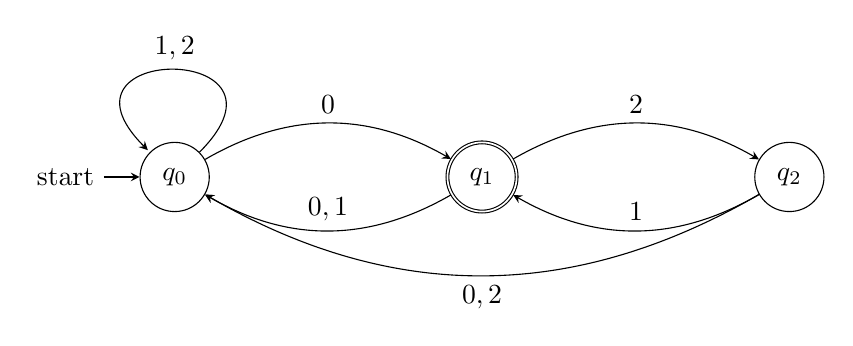
\begin{tikzpicture}[->,>=stealth] 

\node [state,initial] (q0){$q_0$};
\node[state,accepting,right = 3cm of q0](q1){$q_1$};
\node[state,right = 3cm of q1](q2){$q_2$};

\path (q0) edge [above,bend left] node{$0$}(q1);
\path (q2) edge [above,bend left] node{$1$}(q1);
\path (q1) edge [above,bend left] node{$2$}(q2);
\path(q1) edge [above,bend left]  node{$0,1$}(q0);
\path(q2) edge [below,bend left]  node{$0,2$}(q0);
%loop

\path (q0) edge [above,loop] node{$1,2$}(q0);

%\path (q1) edge[bend left, above]  node {$ P_2,P_3,...P_m$} (q0);

%\path (q2) edge[bend left, above]  node {$ P_1,P_3,...,P_m$} (q0);
%\path (qm) edge[bend left, below]  node {$P_1,P_2,...,P_{m-1}$} (q0);


%\node[state,accepting](qm){$q_m$};
\end{tikzpicture}
 %%%%%%%%%%%%%%%%%%% First Question%%%%%%%%%%%%%%%%%%%%%%%%
 
 
 
 %%%%%%%%%%%%%%%%%%% Second Question%%%%%%%%%%%%%%%%%%%%%%%
 
\paragraph{\Large{Question 2\\ \\}}
Algorithm 1 returns a result in the time proportional to \me{O(|T| |S|)}. Discuss the computation time of your automaton.\newline
\\ In the worst case the automata will have \me{O(|T| |S|)} complexity. We know this because the tree diagram of the Automata reads at most \me{|T|}. For each of these readings there are \me{|S|} possible states to consider or that it compares.Thus the automata has the same time complexity as the algorithm. 
\newline \newline
In tree diagram below explores all of the possible text inputs from {$T_1$} all the way to {$T_n$}. For the corresponding pattern we induce a empty transition to the acceptance state if the pattern. \\ We consider every possible comparison up to $P_m$. Note that the last $P_m$ is not necessarily the only comparison we do of $P_m$, there may be multiple comparisons in between the tree diagram. \\
\begin{tikzpicture}[->,>=stealth] 




\node[state](a1) {$P_1$};
\node[state,right = 3cm of a1](a2) {$P_2$};
\node[state,above = 3cm of a2](s) {$$};
\node[state,right = 3cm of a2](am) {$P_m$};
\node[state,accepting,right = 1cm of a1] (acc){$$};
\path (s)  edge[left] node{$T_1$} (a1);
\path (s)  edge[left] node{$T_1$} (a2);
\path (s)  edge[left] node{$T_1$} (am);
\path (a2)  edge[above,dotted,thick] node{$$} (am);
\path (a1)  edge[above] node{$\epsilon$} (acc);


\node[state,below = 2cm of a1](b2) {$P_2$};
\node[state,left = 1cm of b2](b1) {$P_1$};
\node[state,right = 2cm of b2](bm) {$P_m$};
\node[state,accepting,right = 0.5cm of b2](acc) {$$};
\path (a1)  edge[left] node{$T_2$} (b1);
\path (a1)  edge[left] node{$T_2$} (b2);
\path (a1)  edge[left] node{$T_2$} (bm);
\path (a1)  edge[above,dotted,thick] node{$$} (bm);
\path (b2)  edge[above] node{$\epsilon$} (acc);


\node[state,below = 4cm of b2](tm) {$P_m$};
\node[state,accepting,right = 0.5cm of tm](acc) {$$};
\node[state,below = 5cm of a2] (g){$P_m$};
\node[state,below= 5cm of am] (h){$P_m$};
\path (b2)  edge[left,dotted,thick] node{$T_n$} (tm);
\path (tm)  edge[above] node{$\epsilon$} (acc);
\path (a2)  edge[left,dotted,thick] node{$$} (g);
\path (am)  edge[left,dotted,thick] node{$$} (h);





\end{tikzpicture}


 %%%%%%%%%%%%%%%%%%% Second Question%%%%%%%%%%%%%%%%%%%%%%%

\end{document}